\vfill
\begin{block}{Big picture}
  \begin{center}
  {\large How do you deploy a high accuracy classifier starting with zero training examples?}\\
  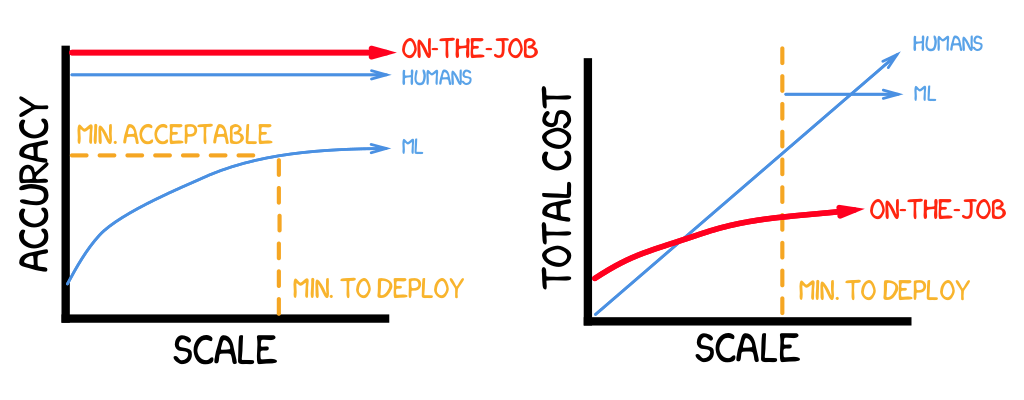
\includegraphics[width=0.8\columnwidth]{graph}
  \end{center}

\end{block}
\vfill

\begin{block}{What is on-the-job learning?}
  \begin{itemize}
    \item 
  \textbf{On-the-job learning} allows a system to query the crowd for labels on the uncertain parts of an input as it arrives \textbf{before} making a prediction.

%  \begin{center}
%    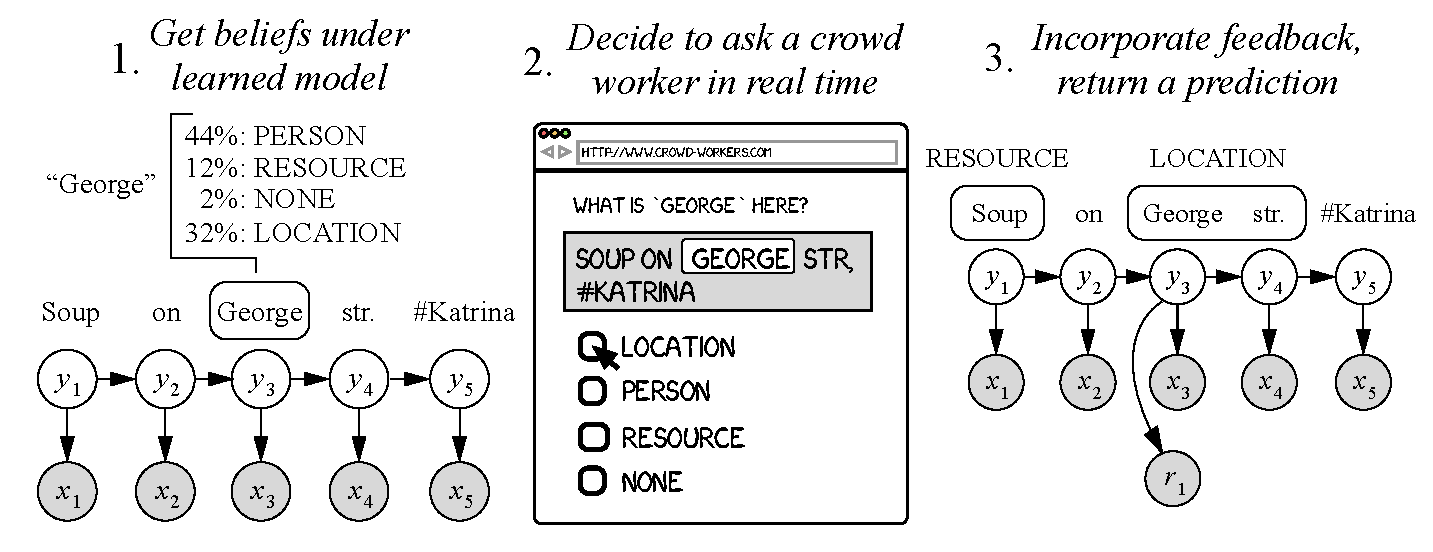
\includegraphics[width=0.8\columnwidth]{intro-banner}
%  \end{center}

    \item Can \textbf{maintain accuracy on difficult examples} by asking the crowd for assistance.
    \item \textbf{Reduces costs} on simpler examples by learning a better prediction model online (on-the-job).
    \item User specifies a base prediction model and how to trade off accuracy, cost and latency. 
    \item System optimizes for utility using ideas from game playing and Bayesian decision theory.
  \end{itemize}
\end{block}
\vfill

\begin{block}{Related work}
  \begin{tabular}{p{0.54\columnwidth} p{0.39\columnwidth}}
    \textbf{Area} & \textbf{Paradigm} \\ \midrule
    \textbf{Online active learning}
      chooses the most informative examples to label \emph{after} classification. 
      Impossible to maintain high accuracy initially.
      & 
      \begin{center}
      \tikz{
      \node[draw, fill=palette2, rectangle, scale=0.7] (inp) {\textsc{Input}};
      \node[draw, fill=palette3, rectangle, right, scale=0.7] (pred) at ($(inp.east)$) {\textsc{Predict}};
      \node[draw, fill=palette5, rectangle, right, scale=0.7] (label) at ($(pred.east)$) {\textsc{Label}};
      \node[draw, fill=palette1, rectangle, right, scale=0.7] (learn) at ($(label.east)$) {\textsc{Learn}};
      }
      \end{center}
      \\
      %Input, Predict, Label, Learn \\
    \textbf{Active classification} 
    learns a static policy from a labelled dataset to choose features to query at test time.
      & 
      \begin{center}
      \tikz{
      \node[draw, fill=palette2, rectangle, scale=0.7] (inp) {\textsc{Input}};
      \node[draw, fill=palette5, rectangle, right, scale=0.7] (label) at ($(inp.east)$) {\textsc{Label}$^*$};
      \node[draw, fill=palette3, rectangle, right, scale=0.7] (pred) at ($(label.east)$) {\textsc{Predict}};
%      \node[draw, fill=palette1, rectangle, right, scale=0.7] (learn) at ($(pred.east)$) {\phantom{Learn}};
      }
      \end{center}
      \\
    \textbf{On-the-job learning}
    combines advantages of both the above methods. Note,
Legion:AR \citep{lasecki2013real} studied the user interface
      aspects of on-the-job learning, while we study the machine learning
      aspects of it.
      & 
      \begin{center}
      \tikz{
      \node[draw, fill=palette2, rectangle, scale=0.7] (inp) {\textsc{Input}};
      \node[draw, fill=palette5, rectangle, right, scale=0.7] (label) at ($(inp.east)$) {\textsc{Label}};
      \node[draw, fill=palette3, rectangle, right, scale=0.7] (pred) at ($(label.east)$) {\textsc{Predict}};
      \node[draw, fill=palette1, rectangle, right, scale=0.7] (learn) at ($(pred.east)$) {\textsc{Learn}};
      }
      \end{center}
      \\
  \end{tabular}


  %\begin{itemize}
  %  \item Legion:AR \citep{lasecki2013real} study the user interface
  %    aspects of on-the-job learning, while we study the machine learning
  %    aspects of it.



  %  \item \textbf{Online active learning}: The key distinction from
  %    online active learning is that in on-the-job learning, (noisy
  %    partial) labels are obtained \emph{before} a prediction is made.
  %    \todo{figure}.
  %  \item \textbf{Active classification}: Active classification algorithms learns a static policy from a labelled dataset for when certain features should be queried which does not change at test time, whereas on-the-job learning continuously updates itself, 
  %\end{itemize}
\end{block}
\vfill

